\chapter{Resultados Parciais: Segunda contribui\c{c}\~ao}
\section{Feixes Vectoriais puramente propagantes com simetria azimutal}
\subsection{Metodologias matem\'aticas para a constru\c{c}\~ao de feixes vetoriais}
Um feixe electromagn\'etico pode-se considerar paraxial quando al\'em de cumprir as propriedades de paraxialidade do caso escalar possu\'ia componentes do campo transversal muito maiores que a componente longitudinal, portanto o caso de feixe eletromagn\'etico n\~ao paraxial \'e mais complexo porque al\'em de possuir as dificuldades do caso escalar apresenta tamb\'em o problema de polariza\c{c}\~ao do feixe.\\
No caso n\~ao paraxial ocorre que as componentes transversais do campo s\~ao, em geral, da ordem de grandeza (talvez at\'e menores) do que a componente longitudinal. Assim, no caso vetorial, uma dificuldade adicional est\'a relacionada com a polariza\c{c}\~ao do campo. Neste sentido forneceremos um m\'etodo matem\'atico para obter solu\c{c}\~oes das equa\c{c}\~oes de Maxwell descrevendo a evolu\c{c}\~ao de feixes n\~ao paraxiais.\\
As equa\c{c}\~oes de Maxwell no espa\c{c}o livre sem cargas nem densidade de corrente ($\rho=\vec{J}=0$) s\~ao: 
\begin{eqnarray}
\vec{\nabla}\cdot\vec{E}&=&0 \label{eq001}\\
\vec{\nabla}\times\vec{E}&=&-\frac{\partial}{\partial t}\vec{B}\label{eq002}\\
\vec{\nabla}\cdot\vec{B}&=&0\label{eq003}\\
\vec{\nabla}\times\vec{B}&=&\mu_0\varepsilon_0\frac{\partial}{\partial t}\vec{E}\label{eq004}
\end{eqnarray}
Onde $\varepsilon_0$, $\mu_0$ s\~ao a permissividade e a permeabilidade  no v\'acuo respectivamente.\\
%****************************************************************************************************************************
\subsection{M\'etodo das derivadas parciais}
Vamos supor que desejamos um feixe eletromagn\'etico com polariza\c{c}\~ao:
\begin{equation}\label{eq01}
\vec{E}=E_{y}\hat{y} + E_z\hat{z}
\end{equation}
Substituindo (\ref{eq01}) em (\ref{eq001}) temos:
\begin{eqnarray}
 \left(\hat{x}\frac{\partial}{\partial x}+\hat{y}\frac{\partial}{\partial y}+\hat{z}\frac{\partial}{\partial z}\right)\cdot (E_{y}\hat{y}+E_z\hat{z}) & = & 0 \nonumber\\
 E_z & = & -\frac{\partial}{\partial y}\int E_{y}dz\label{eq02}
\end{eqnarray}
Seja $\psi$ solu\c{c}\~ao da equa\c{c}\~ao de onda, ent\~ao suas derivadas tamb\'em s\~ao solu\c{c}\~oes da equa\c{c}\~ao de onda. Seja:
\begin{equation}\label{eq03a}
\psi =\int E_y dz
\end{equation}
ent\~ao
\begin{equation}\label{eq03}
E_y= \frac{\partial}{\partial z}\psi
\end{equation}
 usando (\ref{eq03a}) em (\ref{eq02}) temos:
\begin{equation}\label{eq04}
E_z= -\frac{\partial}{\partial y}\psi
\end{equation}
Seja $\psi$ igual \`a solu\c{c}\~ao da equa\c{c}\~ao de onda dada por (\ref{eqA20}). Por\'em por (\ref{eq03}) e (\ref{eq04}) as componentes do campo el\'etrico $E_y$ e $E_z$ tamb\'em s\~ao solu\c{c}\~oes da equa\c{c}\~ao de onda. Substituindo (\ref{eqA20}) em (\ref{eq03}) e (\ref{eq04}) temos:
\begin{equation}\label{eq05}
E_y= \exp[-{\rm i}\omega t]\left(\frac{\omega}{c}\right)\sum\limits_{n=-\infty}^{\infty}R_n  (n \pi +\frac{\omega}{c} z )  \left(\frac{\cos[h]}{h^2} -\frac{\sin\left[h\right]}{h^3}\right)
\end{equation}
\begin{equation}\label{eq06}
E_z= \exp[-{\rm i}\omega t]\left(\frac{\omega^2}{c^2}\right)\sum\limits_{n=-\infty}^{\infty}R_n y \left(\frac{\sin[h]}{h^3}-\frac{\cos[h]}{h^2}\right)
\end{equation}
onde $h$ foi definido em (\ref{eqs3}):
$$ h = \sqrt{\frac{\omega^2}{c^2}\rho^2+(z\frac{\omega}{c}+\pi n)^2}$$
Al\'em de obter o campo el\'etrico tamb\'em podemos obter a meia temporal do vetor de Poynting $<\vec{S}>$. Notando que a parte temporal do feixe \'e $ \exp[-{\rm i}\omega t]$ de (\ref{eq002}) temos:
\begin{eqnarray}
 \vec{\nabla}\times\vec{E} & = &{\rm i}\omega \vec{B}\nonumber\\
     \vec{B} & = &  -\frac{ {\rm i}}{\omega} \left(\vec{\nabla}\times\vec{E}\right)  \label{eq07}
\end{eqnarray}
A meia temporal do vetor de Poynting \'e:
\begin{equation}\label{eq08}
     <\vec{S}>  =   \frac{1}{2}Re\left[ \vec{E}\times\vec{H}^{*} \right]
\end{equation}
com $\vec{H}=\vec{B}/\mu_{0}$.\\
%e a intensidade:
%\begin{equation}\label{eq08}
 %  \langle \vec{S} \rangle =   \frac{1}{2\mu_0}\Re e\left( \vec{E}\times\vec{B}^{*} \right)
%\end{equation}
Substituindo (\ref{eq05}) e (\ref{eq06}) em (\ref{eq07}) temos:
\begin{equation}\label{eq09}
     \vec{B}  =  B_x\hat{x} +B_y\hat{y}+B_z\hat{z}
\end{equation}
Substituindo $\vec{E}$ e $\vec{H}$ em (\ref{eq08}) podemos obter a meia temporal do vetor de Poynting $<\vec{S}>$.\\
%\begin{eqnarray}
% B_x & =&-{\rm i}\exp[-{\rm i}\omega t]\left(\frac{\omega}{c^2}\right)\sum\limits_{n=-\infty}^{\infty}A_n\left[\left(y ^2\frac{\omega^2}{c^2} + [n \pi+\frac{\omega}{c} z] ^2\right)\left(\frac{3 \cos[h]}{ h^4}-\frac{3 \sin[h]}{h^5}+\frac{\sin[h]}{h^3}\right)-2\left(\frac{\cos[h]}{h^2}-\frac{\sin[h]}{h^3}\right) \right]\label{eq010} \\
 %B_y & = & -{\rm i}\exp[-{\rm i}\omega t]\left(\frac{\omega^3}{c^4}\right)\sum\limits_{n=-\infty}^{\infty}A_n x y \left(\frac{3 \sin[h]}{ h^5}-\frac{3 \cos[h]}{ h^4}-\frac{\sin[h]}{ h^3}\right)  \label{eq011} \\
%  B_z & = &-{\rm i} \exp[-{\rm i}\omega t]\left(\frac{\omega^2}{c^3}\right)\sum\limits_{n=-\infty}^{\infty}A_n x \left(n \pi +\frac{\omega }{c}z\right) \left(\frac{3\sin [h]}{h^5}-\frac{3\cos [h]}{h^4}-\frac{\sin [h]}{ h^3}\right) \label{eq012}
%\end{eqnarray}
%*******************************************************************************
%*******************************************************************************
\begin{figure}[h]
\centering
\subfigure[]{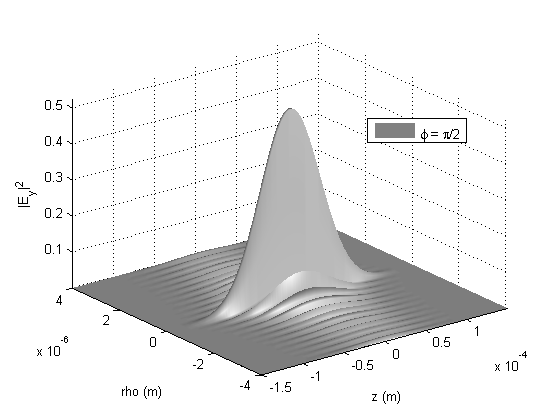
\includegraphics[scale=0.32]{vecgasEy1a.png}}
\centering
\subfigure[]{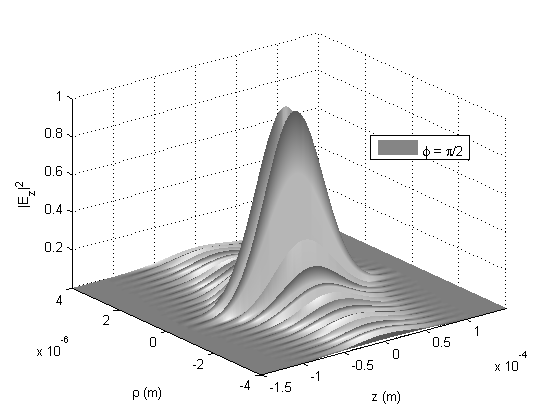
\includegraphics[scale=0.32]{vecgasEz1a.png}}
\centering
\subfigure[]{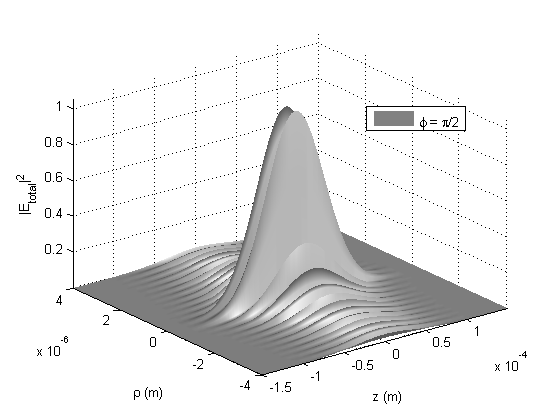
\includegraphics[scale=0.32]{vecgasEtotal1a.png}}\\
\centering
\subfigure[]{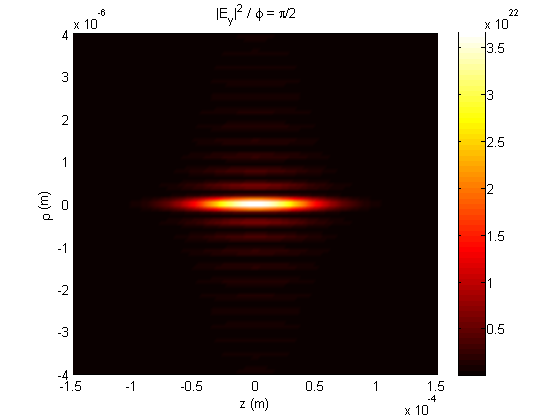
\includegraphics[scale=0.32]{vecgasEy1b.png}}
\centering
\subfigure[]{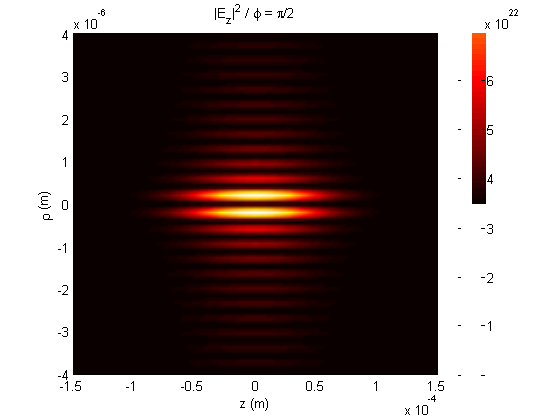
\includegraphics[scale=0.32]{vecgasEz1b.png}}
\centering
\subfigure[]{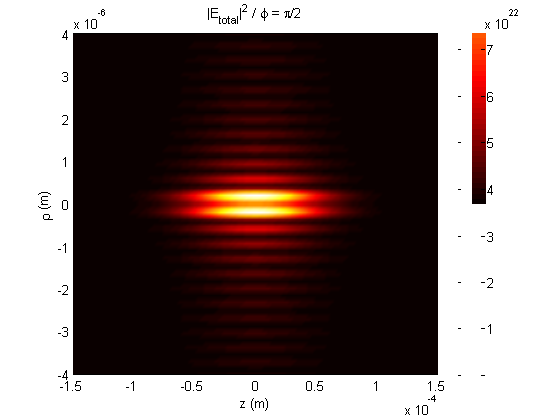
\includegraphics[scale=0.32]{vecgasEtotal1b.png}}\\
\centering
\subfigure[]{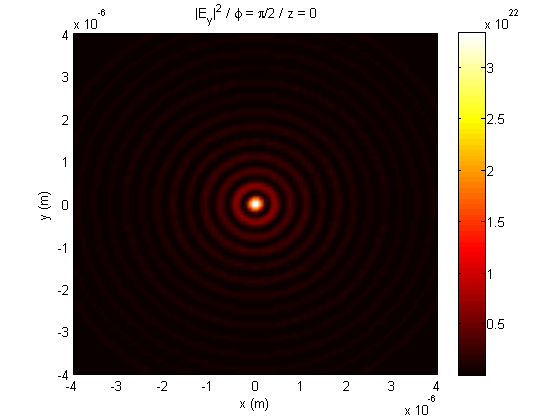
\includegraphics[scale=0.32]{vecgasEy1c.png}}
\centering
\subfigure[]{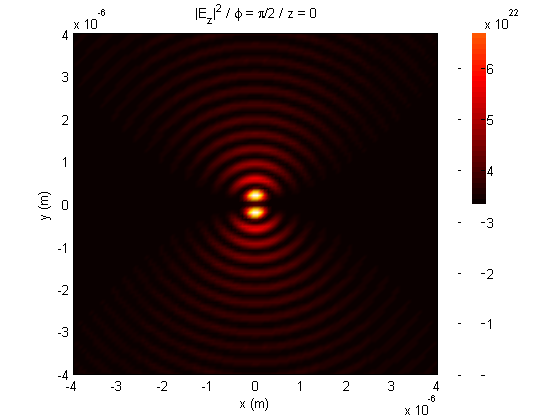
\includegraphics[scale=0.32]{vecgasEz1c.png}}
\centering
\subfigure[]{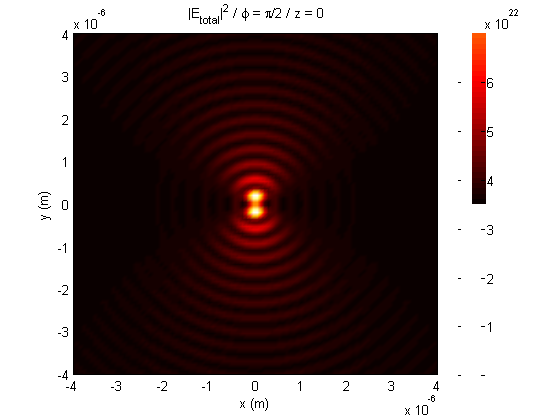
\includegraphics[scale=0.32]{vecgasEtotal1c.png}}
\caption{(a)-(c) Padr\~oes de intensidade 3D das componentes do campo el\'etrico do feixe n\~ao paraxial para $\phi=\pi/2$, (a) componente $E_y$, (b) componente $E_z$ e (c) campo el\'etrico total. (d)-(f) Proje\c{c}\~ao ortogonal da intensidade do feixe gaussiano no plano $(\rho,z)$.  (g)-(i) Proje\c{c}\~oes ortogonais das componentes da intensidade do feixe gaussiano no plano $(x,y)$ para $z=0$. }
\label{fig5}
\end{figure}
%*******************************************************************************
%*******************************************************************************
Com o objetivo de a validar a metodologia proposta, foi estudado um feixe eletromagn\'etico com polariza\c{c}\~ao (\ref{eq01}), onde suas componentes s\~ao dadas por (\ref{eq05}) e (\ref{eq06}). Os valores dos coeficientes $R_n$ em (\ref{eq05}) e (\ref{eq06}) s\~ao dados em (\ref{eqA18}). Nosso espectro $S(k_z)$ n\~ao paraxial foi o mesmo usado em (\ref{ga1}), ou seja, um espectro n\~ao paraxial do tipo gaussiano (ver Figura \ref{fig3}(a)).\\
Na Figura \ref{fig5}(a,b) s\~ao apresentados os padr\~oes de intensidade 3D das componentes transversais do campo el\'etrico $E_y$  e $E_z$ respectivamente  e na Figura \ref{fig5}(c) \'e apresentado o padr\~ao de intensidade do campo el\'etrico total $\vec{E}$.  Os graficos obtidos s\~ao solu\c{c}\~oes exatas das equa\c{c}\~oes de Maxwell e s\~ao obtidos de (\ref{eq05}) e (\ref{eq06}) para $\phi=\pi/2$ e usando $y = \rho\sin\phi$. Os feixes produzidos n\~ao possuem simetria azimutal e s\~ao propagantes.\\
Nas Figuras \ref{fig5}(d,e,f) s\~ao apresentados as proje\c{c}\~oes ortogonais do feixe vetorial no plano $(\rho,z)$.  O feixe eletromag\'etico obtido prov\^em do espetro n\~ao paraxial e possui componentes com mesma ordem de grandeza. O feixe resultante \'e solu\c{c}\~ao anal\'itica exata das equa\c{c}\~oes de Maxwell.\\
Nas Figuras \ref{fig5}(g,h,i) s\~ao apresentadas as proje\c{c}\~oes ortogonais do feixe vetorial no plano $(x,y)$ com $z=0$ em (\ref{eq05}) e (\ref{eq06}).\\
%***************************************************************************************************************
\subsection{M\'etodo do potencial vetor}
Como $\vec{\nabla}\times\vec{B}=0$ (\ref{eq003}), ent\~ao existe um vetor $\vec{A}$ tal que:
\begin{equation}\label{eq006}
\vec{B}=\vec{\nabla}\times\vec{A}
\end{equation}
Substituindo (\ref{eq006}) em (\ref{eq002}) e operando obtemos:
\begin{equation}\label{eq007}
\vec{\nabla}\times(\vec{E}+\frac{\partial}{\partial t}\vec{A})=0
\end{equation}
de (\ref{eq007}) deduzimos que o campo vetorial $\vec{E}+\frac{\partial}{\partial t}\vec{A}$ \'e um campo conservativo \cite{Lya:32}\cite{Lya:33}. Portanto existe uma fun\c{c}\~ao escalar $V$, tal que:
\begin{eqnarray}
-\nabla V &=& \vec{E}+\frac{\partial}{\partial t}\vec{A}\nonumber\\
\vec{E}&=&-\nabla V- \frac{\partial }{\partial t}\vec{A} \label{eq008}
\end{eqnarray}
O n\'umero de solu\c{c}\~oes para $\vec{A}$ e $V$ s\~ao infinitos, por\'em vamos obter as equa\c{c}\~ao que $\vec{A}$ e $V$ devem atender.\\
Usando (\ref{eq008}) em (\ref{eq001}) temos:
\begin{equation}\label{eq009}
\vec{\nabla}^2V+\frac{\partial}{\partial t}(\vec{\nabla}\cdot\vec{A}) = 0
\end{equation}
Substituindo (\ref{eq006}) e (\ref{eq008}) em (\ref{eq004}), para $c^2=1/\mu_0\varepsilon_0$, temos:
\begin{equation}\label{eq0010}
0=-\nabla[\vec{\nabla}.\vec{A} + \frac{1}{c^2}\frac{\partial }{\partial t}V]+ \vec{\nabla}^2\vec{A}-\frac{1}{c^2}\frac{\partial^2}{\partial t^2}\vec{A}
\end{equation}
escolhemos o gauge de Lorentz igual a:
\begin{equation}\label{eq0011}
\vec{\nabla}\cdot\vec{A}=- \frac{1}{c^2}\frac{\partial }{\partial t}V
\end{equation}
Finalmente usando (\ref{eq0011}) em (\ref{eq0010}) e em (\ref{eq009}) obtemos um sistema de equa\c{c}\~oes que envolve a $\vec{A}$ e $V$:
\begin{eqnarray}
\nabla^{2}\vec{A} - \frac{1}{c^2}\frac{\partial ^2}{\partial t^2}\vec{ A}&=& 0\label{eq0012}\\
\nabla^{2}V - \frac{1}{c^2}\frac{\partial ^2}{\partial t^2}V &=& 0\label{eq0013}
\end{eqnarray}
Para obter um feixe com poliza\c{c}\~ao $\vec{E}=E_{\rho}\hat{\rho}+E_{z}\hat{z}$, se escolheu:
\begin{equation}\label{eq0016a}
 \vec{A}(\rho,z,t)=\hat{z}A_z(\rho,z,t)
\end{equation}
com $A_z(\rho,z,t)$ igual a solu\c{c}\~ao anal\'itica da equa\c{c}\~ao de onda mostrada em (\ref{eqA20}). A solu\c{c}\~ao (\ref{eq0016a}) pode ser escrita na forma harm\^onica como:
\begin{equation}\label{eq0016b}
A_z(\rho,z,t)=A_z(\rho,z)\exp[-{\rm i}\omega t] 
\end{equation}
O $V$ pode ser obtido a partir do $\vec{A}$. Substituindo (\ref{eq0016b}) em (\ref{eq0011}), temos:
\begin{eqnarray}
 (\frac{1}{\rho}\frac{\partial}{\partial \rho}(\rho)\hat{\rho}+\frac{1}{\rho}\frac{\partial}{\partial\phi}\hat{\phi}+\frac{\partial}{\partial z}\hat{z})\cdot \hat{z}A_z(\rho,z)\exp[-{\rm i}\omega t] & = & -\frac{1}{c^2}\frac{\partial}{\partial t} V \nonumber\\
 \frac{\partial }{\partial z} A_z(\rho,z)\exp[-{\rm i}\omega t] & = &  -\frac{1}{c^2}\frac{\partial}{\partial t} V \nonumber\\
   V(\rho,z,t)& = & -c^2\frac{\partial }{\partial z}A_z(\rho,z)\int\exp[-{\rm i}\omega t] dt \nonumber\\
 &=& -{\rm i}\frac{c^2}{\omega} \frac{\partial }{\partial z} A_z(\rho,z)\exp[-{\rm i}\omega t]\nonumber\\
 V(\rho,z,t)&=&  -{\rm i}\frac{c^2}{\omega} \frac{\partial }{\partial z}A_z(\rho,z,t)
\label{eq0016}
\end{eqnarray}
Substituindo $A_z(\rho,z,t)$ igual a solu\c{c}\~ao anal\'itica da equa\c{c}\~ao (\ref{eqA20}) em (\ref{eq0016}), temos:
\begin{equation}\label{eq0017}
 V(\rho,z,t)= {\rm i}\exp[-{\rm i}\omega t]\sum\limits_{n=-\infty}^{\infty}R_n  (c n \pi +\omega z )  \left(\frac{\sin\left[h\right]}{h^3}-\frac{\cos[h]}{h^2}\right)
\end{equation}
Onde $h$ foi definido em ($\ref{eqs3}$):
$$ h = \sqrt{\frac{\omega^2}{c^2}\rho^2+(z\frac{\omega}{c}+\pi n)^2} $$
Substituindo $V$ de (\ref{eq0017}) e $\vec{A}$ (com $A_z(\rho,z,t)$ dado em $\ref{eqA20}$) em (\ref{eq008}) obtemos o campo el\'etrico com componentes:
\begin{equation}\label{eq0020}
E_{\rho}= {\rm i}\left(\frac{\omega^2}{c^2}\right)\exp[-{\rm i}\omega t]\sum\limits_{n=-\infty}^{\infty}R_n(c n \pi +\omega z) \rho  \left(\frac{3 \sin[h]}{ h^5} -\frac{3\cos[h]}{ h^4}-\frac{\sin[h]}{h^3}\right) 
\end{equation}
\begin{align}
\nonumber E_z&=& {\rm i}\exp[-{\rm i}\omega t]\sum\limits_{n=-\infty}^{\infty}R_n\left[\omega (\frac{\cos[h]}{h^2}-\frac{\sin[h]}{h^3})+\frac{\omega}{c^2} (c n \pi +\omega z)^2(\frac{3 \sin[h]}{h^5}-\frac{3\cos[h]}{h^4}-\frac{ \sin[h]}{h^3})\right.\\
 & & + \left.\omega (\frac{\sin[h]}{h} )\right]\label{eq0021}
\end{align}
substituindo $\vec{A}$ (com $A_z(\rho,z,t)$ dado em $\ref{eqA20}$) em (\ref{eq006}), obtemos o campo magn\'etico:
\begin{equation}\label{eq0022}
\vec{B}= \hat{\phi}\exp[-{\rm i}\omega t]\frac{\omega^2}{c^2}\sum\limits_{n=-\infty}^{\infty}R_n \rho \left(\frac{\sin\left[h\right]}{h^3}-\frac{\cos[h]}{h^2}\right)
\end{equation}
Repare que a dire\c{c}\o do campo magn\'etico \'e s\'o no $\phi$, portanto se aplicamos o teorema da dualidade \cite{Lya:21} podemos obter feixes vetoriais polarizados s\'o em $\phi$. 
